\chapter{Experiments}
\section{Motivation}
With the ultimate aim of leveraging equivariance for model-based RL. A series of Experiments were carried out, sequentially, to investigate how to exploit known symmetries in a model based environment.

Model-Based RL, is inherently more complex than Actor-Critic or Value based methods, as not only does a policy need to be learned, but also a model of the environment dynamics must also be learned.

Due to the increased complexity of Model based methods, and the benefit of implementing existing methods, while also providing a baseline for further experimentation a model-free implementation was created.

\section{Baseline}
The baseline that was chosen was a proximal policy optimization agent from PureJaxRL,~\cite{lu2022discovered}. This baseline provides a training framework, that trains a single agent concurrently on multiple environments.

The Training regime is outlined below in pseudo code.
\begin{algorithm}
	\caption{PureJaxRL PPO Agent Training Structure}
	\begin{algorithmic}
		\State Initialize Agent: Actor-Critic $\pi_\theta$, $v_\phi$
		\State Initialize Replay Buffer: $\mathcal{D}$
		\For{Num Updates}
		\State Gain Experience For Num Timestep
		\State Store trajectories: $\mathcal{D}$.append($(S, A, S', R))$
		\State Calculate GAE Estimate From timesteps
		\For{ Num Epochs}
		\State{ Split GAE Estimates into minibatches}
		\State{ Mini-Batch SGD with Adam on $\pi_\theta, v_\phi$}
		\Comment{ See~\ref{alg:PPO} for Losses to optimize}
		\EndFor
		\EndFor
		\State Returns($\mathcal{D}$)

	\end{algorithmic}
\end{algorithm}

\section{Equivariant Actor-Critics}
\subsection{CartPole}

To form an equivariant network to the group structure of CartPole the actor network must be equivariant to both the identity and inversion operator. This report provides structures for equivariant G-CNNs for both Cart-pole and Catch, that can easily be extended to other environments with known discrete symmetries.


In this section, the outline for the network design is described. In the Catch section, a more detailed description of how to extend the procedure to other Groups is outlined.
The Group for Cart-pole contains two unique elements, in both state and action space. In state space the inversion and identity operator $r, e$ are,
\begin{equation}
	\ell^\mathcal{S}_e =
	\begin{pmatrix}
		1 & 0 & 0 & 0 \\
		0 & 1 & 0 & 0 \\
		0 & 0 & 1 & 0 \\
		0 & 0 & 0 & 1 \\
	\end{pmatrix},
	\ell^\mathcal{S}_r =
	\begin{pmatrix}
		-1 & 0  & 0  & 0  \\
		0  & -1 & 0  & 0  \\
		0  & 0  & -1 & 0  \\
		0  & 0  & 0  & -1 \\
	\end{pmatrix}.
\end{equation}
Then the action space, the inversion and identity operator are,
\begin{equation}
	\ell^\mathcal{A}_e =
	\begin{pmatrix}
		1 & 0 \\
		0 & 1 \\
	\end{pmatrix},
	\ell^\mathcal{A}_r =
	\begin{pmatrix}
		0 & 1 \\
		1 & 0 \\
	\end{pmatrix}.
\end{equation}
Thus, to parameterize an equivariant actor network, the network $\pi_\theta$ must satisfy,
\begin{equation}
	\pi_\theta(\ell^\mathcal{S}_e s) = \ell^\mathcal{A}_e \pi_\theta(s),
\end{equation}
\begin{equation}
	\pi_\theta(\ell^\mathcal{S}_r s) = \ell^\mathcal{A}_r \pi_\theta(s),
\end{equation}
Because the operation on the state space is equivariant to odd functions, the actor network, a simple solution is to use a network with only odd operations, i.e. $\tanh$ activation and no biases for all the of the hidden representations. This ensures that the network is equivariant to the inversion operator. Then we use a group convolution layer to map between representations.

The full network can then be thought of as a composition of $f_\theta : \mathcal{S} \rightarrow \mathbb{R}^{|H|}$, an odd embedding MLP and $gc_\theta: \mathbb{R}^{|H|} \rightarrow \mathbb{R}^{\mathcal{A}}$ a group convolution layer that "lifts" the equivariance to the action space. As such the parametric policy is,
\begin{equation}
	\pi_\theta(s) = gc_\theta(f_\theta(s)).
\end{equation}
The non-trivial equivariance properties of the sub-networks are,
\begin{equation}
	f_\theta(-s) = -f_\theta(s),
\end{equation}
\begin{equation}
	gc_\theta(-x) =
	\begin{pmatrix}
		0 & 1 \\
		1 & 0 \\
	\end{pmatrix}
	gc_\theta(x),
\end{equation}
Where $gc_\theta(x) = [P(A=a_0), P(A=a_1)]$ describes the distribution over the binary actions of Cart-pole.

This G-CNN network for policy learning is the first novel contribution of this report. In comparison to the work of \cite{mondal2020group}, the policy learning G-CNN is fully equivariant, rather than learning action values from an equivariant embedding. Additionally, the network parameterizes a policy directly rather than Q values. Due to the network's end to end equivariance in comparison to the Q-value network proposed by \cite{mondal2020group}, agents parameterized by this network must take the same actions in states that are in the same orbit, which is not the case for the Q-value network which only has an equivariant embedding.

Further, this network architecture has advantages over Symmetrizer networks, \cite{vanderpol2020mdp}, in that it does not require a large matrix inversions to solve for the parameters of the network, while still maintaining the same equivariance qualities.

\subsection{Training Dynamics On the Cart-Pole Benchmark}
The networks structure defined, the benchmark task is to learn an expert policy on the Cart-pole environment. In the default setting Cart-pole has a maximum episode length of 500 interactions. All non-terminal states garner a reward of +1. As such, the maximum episodic return is 500. As in all conventional RL problems, in Cart-pole the aim is to maximize the episodic return of the agent. It is straightforward to find an expert policy in Cart-pole, with conventional deep learning methods, and serves only as an implementation benchmark. For an equivariant network structure to improve the learned policy quality it should approach the goal of 500 episodic return with fewer MDP interactions.

When comparing policy agent's learning dynamics it is not only important that, the agent achieves expertise in the task but also that, the policy learning procedure is stable across many random seeds. Where a random seed is the random initial state that the agent and environment start in. With training stability in mind looking at the worst performing random seeds is informative, as if the algorithm is very sensitive to initialization, then this performance may be heavily affected.

For all the experiments, we leave the critic to be a standard MLP, with no equivariance constraints. This may be a non-optimal setting in terms of performance. Additionally, to ensure that all the agent's learning is stable training is performed across 128 random seeds.

Due to the constraints on the equivariant network structures, it is not always possible to have exactly the same number of parameters exactly in the networks. In cases, where exact parameter count matching all network's depth is held constant and, a width is found such that the parameter counts are inside 10\% less.

Below, in fig\ref{fig:cartpole_equivariant_actor}, the episodic return's of three different agents with differing network architectures are plotted. The network's training hyperparameters are all the same, and are those found in the PureJaxRL\cite{lu2022discovered} baselines. The three networks are an MLP baseline from PureJaxRL, an implementation of the Symmetrizer network from \cite{vanderpol2020mdp}, and this report's G-CNN policy network.
\begin{figure}[H]
	\centering
	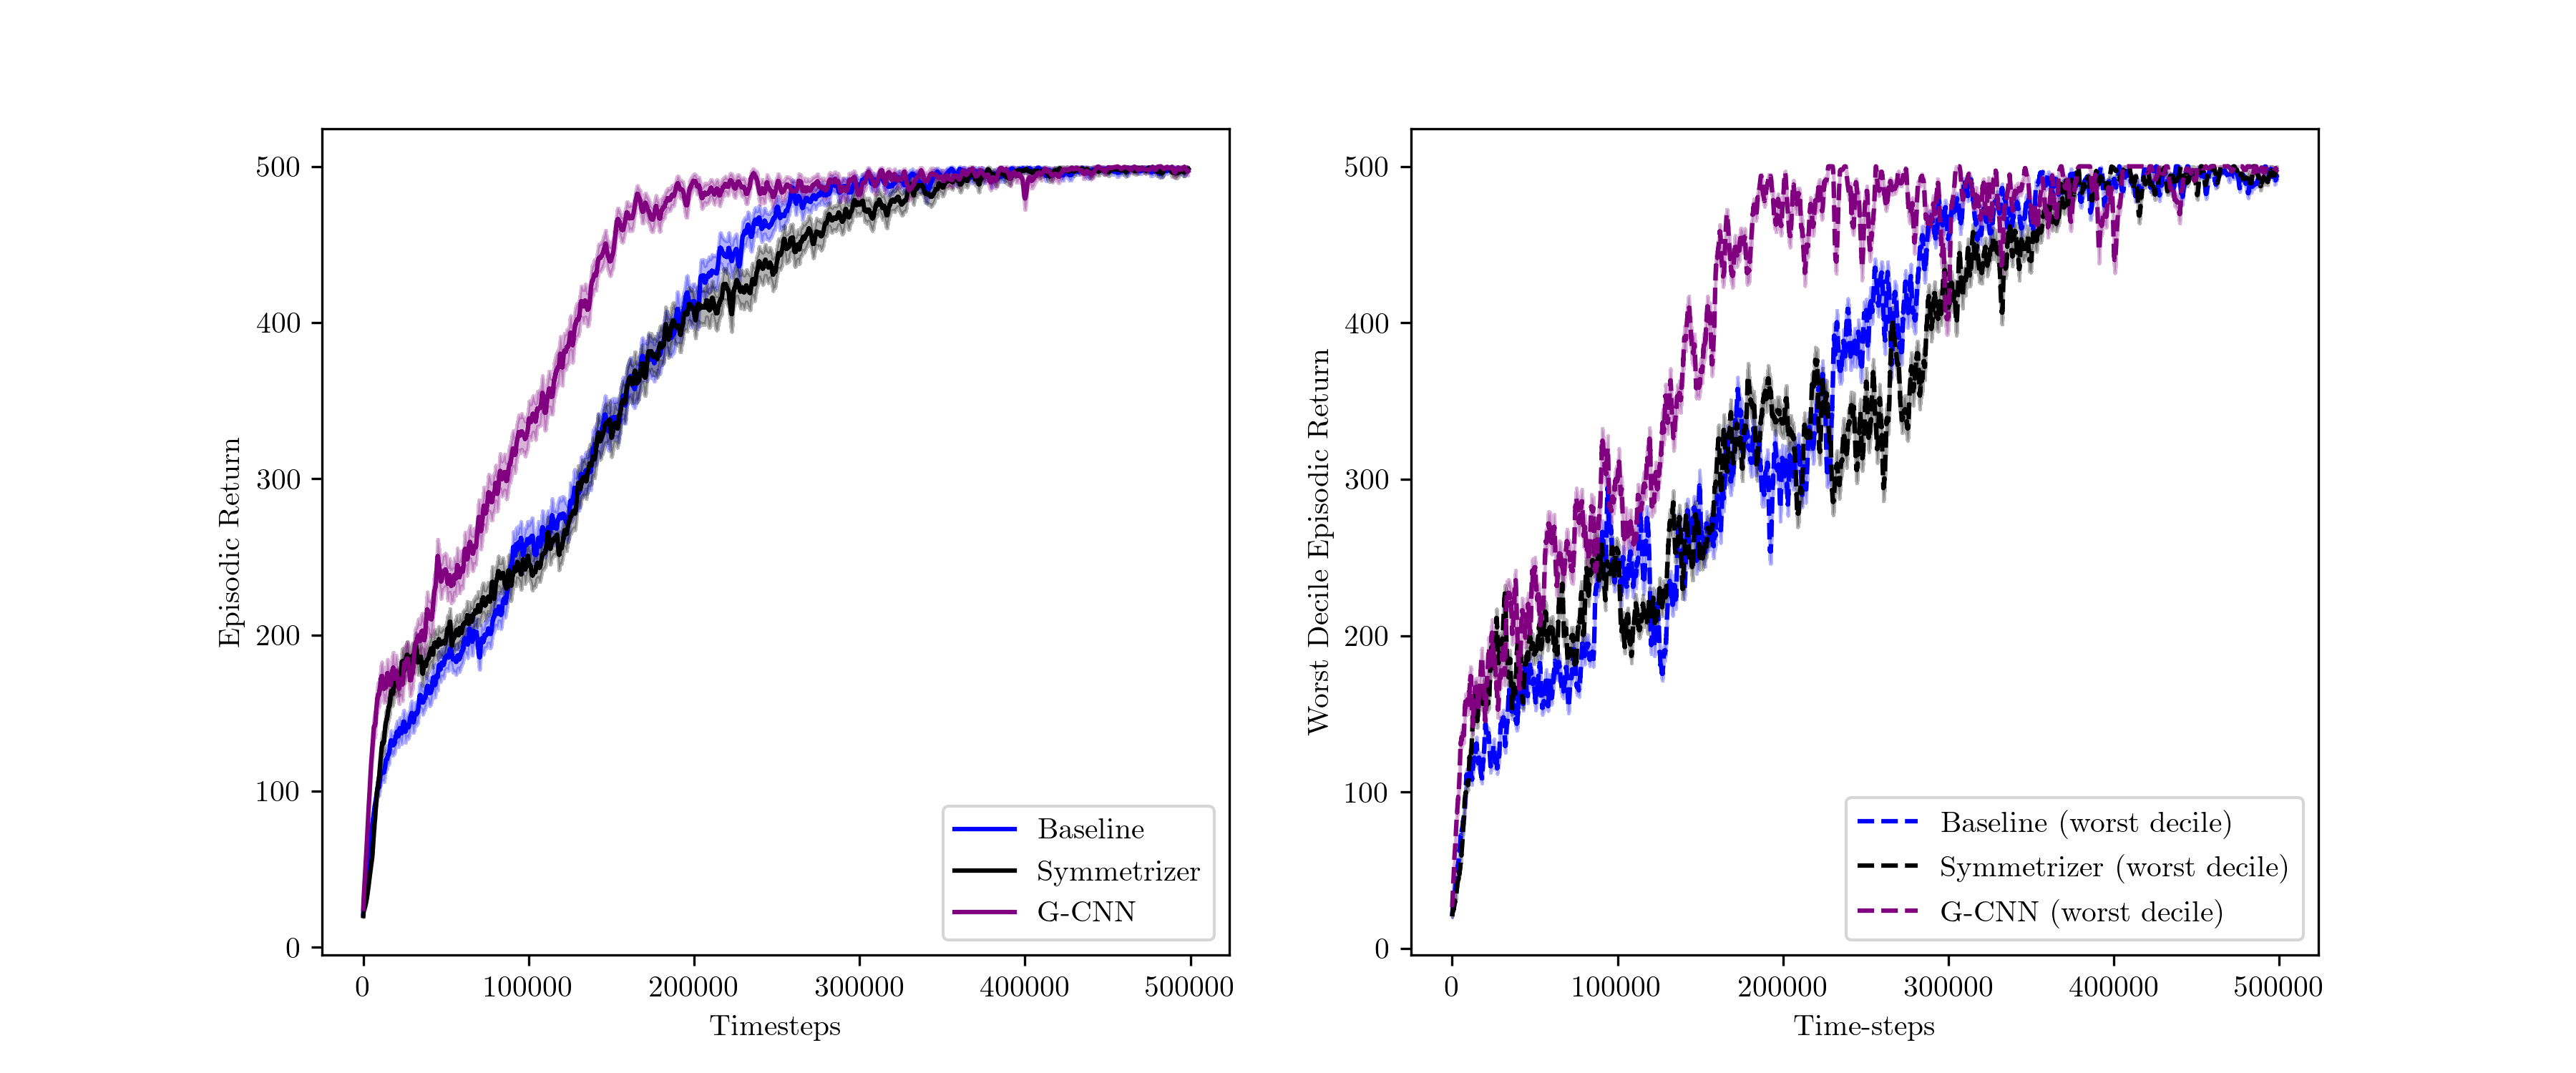
\includegraphics[width=\linewidth]{Figures/cart_pole_returns.png}
	\caption{Left: Mean cumulative episodic returns for the CartPole agents across 128 random seeds plotted against number of experience time-steps in the MDP. Right: The mean cumulative episodic returns of the worst performing 128 random seeds against number of experience time-steps in the MDP. Both of the plots are moving averages, with windows of 10 time-steps. } \label{fig:cartpole_equivariant_actor}
\end{figure}

Both the Symmetrizer and the G-CNN are equivariant to the actions of the $C_2$ group. This equivariance constraint requires a learned policy that respects the inversion symmetry present in Cart-pole. The equivarianc  should improve the sample efficiency of the agent as any learning from one state additionally informs the agent about the agent about the policy for the other state in the orbit. This hypothesis, is supported somewhat by the observed training dynamics. Over the first period of training both the Symmetrizer and the G-CNN, outperform the baseline. The Symmetrizer, does not maintain this performance advantage. Our implementation uses the same network size, as the original paper and the same network hyperparameters. Despite this, the symmetrizer agent fails to learn an expert policy in fewer steps than that of the baseline. The equivariant nature of the network was asserted.

It should be noted that here the mean plus minus two standard deviations is plotted in comparison to the median and upper and lower quartiles of cumulative returns, which is plotted in \cite{vanderpol2020mdp}. The performance of the Symmetrizer, is underwhelming despite the implemented network being checked for equivariance. Further tuning of the hyperparameters may yield performance that improves upon the baseline's returns. However, this was not a primary concern.

The G-CNN does compare favourably with the baseline implementation of an MLP, having slightly fewer parameters. It can be seen that it both converges on average to an expert policy in fewer time-steps but also has a more favourable convergence behaviour in the worst case scenario. This can be seen in the right of Figure \ref{fig:cartpole_equivariant_actor} where, the bottom tenth percentile of cumulative returns, still converges notably faster than that of the baseline.

\begin{table}
	\centering
	\begin{tabular}{|c|c|c|c|}
		\hline
		Time-steps & Baseline     & Symmetrizer          & G-CNN                 \\
		\hline
		$10, 000$  & $102 \pm 5$  & $116 \pm 6$          & $\mathbf{158 \pm 8}$  \\
		$100, 000$ & $260 \pm 10$ & $240 \pm$ 10         & $\mathbf{330 \pm 10}$ \\
		$500,000$  & $497 \pm 1$  & $\mathbf{500 \pm 1}$ & $499 \pm 1$           \\
		\hline
	\end{tabular}
	\caption{Cumulative episodic returns tabulated for the three network architectures. All episodic returns are recorded with confidence intervals of two standard errors across 128 random seeds.}
	\label{tab:actor-critic}
\end{table}

Additionally, the mean Episodic returns across all random seeds are tabulated at $10,000$, $100,000$ and $500,000$ time-steps in Table: \ref{tab:actor-critic}. On closer inspection, the G-CNN agent that includes the equivariant inductive bias vastly outperforms the baseline.

Despite the similar parameter count, because of the structure of the G-CNNs the forward passes are more expensive to compute, requiring the number of group actions times more operations in a forward pass due to the G-CNN architecture. In a problem like Cart-Pole where the networks themselves are small and cheap to evaluate and, the computation can be parallelized, both models train across 128 random seeds in under minute, using the hyperparameters found in the Appendix, on a modern Graphics Card.

\subsection{Catch}







